
\documentclass{beamer}
\usetheme{PaloAlto} %was Warsaw, Singapore, PaloAlto, Ilmenau, Boadilla
% see http://www.pletscher.org/writings/latex/beamerthemes.php
\usepackage{verbatim} %for comments
\usepackage[english]{babel}
\usepackage[latin1]{inputenc}
\usepackage{amsmath}
\usepackage{mathrsfs}
\usepackage{epsfig}
\usepackage{epic}
\usepackage{amsmath}
\usepackage{amsfonts}
\usepackage{amssymb}
\usepackage{latexsym}
\usepackage{multirow}
%\usepackage{algorithm}

\begin{document}

\title{Latte Valuations: Volume and Integration}
\author{}
\date{\today}

\frame{\titlepage}

\section{Volume}
\subsection{Algorithms}



\frame{
\frametitle{Two Flavours}
Latte can compute normalized volumes of polytopes using two different methods:
\begin{enumerate}
\pause
\item The Triangulation Method: Triangulate the polytope into simplices, then use the determinant to find the volume of each simplex.
\pause
\item The Lawrence Method: Triangulate every vertex tangent-cone into simplicial cones and then use a volume formula by Jim Lawrence.
\end{enumerate}
}%frame


\frame{
\frametitle{Volume of a square}
\begin{center}
\resizebox{1.5in}{!}{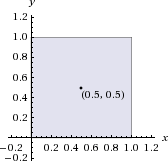
\includegraphics[]{img/unitSquare.png}}
\end{center}
Take the unit square centred at $(1/2, 1/2)$ above; after triangulation, we have two triangles: $\left\lbrace   (0, 0), (1, 0), (1, 1)\right\rbrace$ and $\left\lbrace  (0, 0), (0, 1), (1, 1)\right\rbrace$. Summing the determinant of tiangles' rays and dividing by two give the volume as 1.
}%frame


\frame{
\frametitle{Volume of a square}
\begin{center}
\resizebox{1.5in}{!}{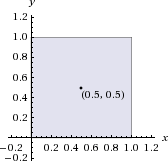
\includegraphics[]{img/unitSquare.png}}
\end{center}
In general, if $\left\lbrace (v_{0i}, v_{1i}, \ldots, v_{di})\right\rbrace  = T_i$ forms a d-simplex such that
the family $\left\lbrace T_1, \ldots, T_k \right\rbrace = \mathcal{T}$ is a triangulation of a d-Polytope, then the volume is given by:

$$
\sum_{T_k\i \in \mathcal{T}} |\det ( v_{1i} - v_{0i}, \ldots, v_{di} - v_{0i})| / d!
$$
}%frame

\subsection{Example}
\frame{
\frametitle{Volume of a square}
For the first step in latte, we need create a file containing he hyperplanes that define the polytope. If $P = \left\lbrace x : Ax < b \right\rbrace$ for some $m \times n$ matrix $A$, then the input file will have the form:

$$
\begin{array}{l l}
 m & n + 1 \\
 \multicolumn{2}{l}{0 \leq b_{i} - a_{i}} \\

\end{array}
$$

where $b_{i}$ is the $i^{th}$ entry of b and $a_i$ is the $i^{th}$ row of $A$.
}%frame


\frame{
\frametitle{Volume of a square}
For our square, its defining hyperplanes are 
$$0 \leq x \leq 1, 0 \leq y \leq 1$$
and so we create a file that contains

\begin{block}<+->{square.latte}
	\begin{tabular}{rrr}
	4 &3 & \\
	0 &1 &0 \\
	1 &-1 &0 \\
	0 &0 &1 \\
	1 &0 &-1 \\
	\end{tabular}
\end{block}

}%frame



\frame{
\frametitle{Volume of a square}
Finally, the command we need is 

\begin{block}<+->{Command:}
./ValuationComputation  --valuation=volume --triangulate square.latte
\end{block}

\begin{block}<+->{Output:}
Volume (using the triangulation-determinant method) \\*
     Answer: 1 (as a fraction) \\*
     Decimal: 1 \\*
     Time: 0.00 sec
\end{block}

}%frame

\frame{
\frametitle{Data Structures}
}%frame

\section{Integration}

\frame{
\frametitle{Algorithm}
\begin{itemize}
\item
\item
\end{itemize}
}%frame	

\frame{
\frametitle{Examples}
}%frame


\end{document}
